\documentclass[1p]{elsarticle_modified}
%\bibliographystyle{elsarticle-num}

%\usepackage[colorlinks]{hyperref}
%\usepackage{abbrmath_seonhwa} %\Abb, \Ascr, \Acal ,\Abf, \Afrak
\usepackage{amsfonts}
\usepackage{amssymb}
\usepackage{amsmath}
\usepackage{amsthm}
\usepackage{scalefnt}
\usepackage{amsbsy}
\usepackage{kotex}
\usepackage{caption}
\usepackage{subfig}
\usepackage{color}
\usepackage{graphicx}
\usepackage{xcolor} %% white, black, red, green, blue, cyan, magenta, yellow
\usepackage{float}
\usepackage{setspace}
\usepackage{hyperref}

\usepackage{tikz}
\usetikzlibrary{arrows}

\usepackage{multirow}
\usepackage{array} % fixed length table
\usepackage{hhline}

%%%%%%%%%%%%%%%%%%%%%
\makeatletter
\renewcommand*\env@matrix[1][\arraystretch]{%
	\edef\arraystretch{#1}%
	\hskip -\arraycolsep
	\let\@ifnextchar\new@ifnextchar
	\array{*\c@MaxMatrixCols c}}
\makeatother %https://tex.stackexchange.com/questions/14071/how-can-i-increase-the-line-spacing-in-a-matrix
%%%%%%%%%%%%%%%

\usepackage[normalem]{ulem}

\newcommand{\msout}[1]{\ifmmode\text{\sout{\ensuremath{#1}}}\else\sout{#1}\fi}
%SOURCE: \msout is \stkout macro in https://tex.stackexchange.com/questions/20609/strikeout-in-math-mode

\newcommand{\cancel}[1]{
	\ifmmode
	{\color{red}\msout{#1}}
	\else
	{\color{red}\sout{#1}}
	\fi
}

\newcommand{\add}[1]{
	{\color{blue}\uwave{#1}}
}

\newcommand{\replace}[2]{
	\ifmmode
	{\color{red}\msout{#1}}{\color{blue}\uwave{#2}}
	\else
	{\color{red}\sout{#1}}{\color{blue}\uwave{#2}}
	\fi
}

\newcommand{\Sol}{\mathcal{S}} %segment
\newcommand{\D}{D} %diagram
\newcommand{\A}{\mathcal{A}} %arc


%%%%%%%%%%%%%%%%%%%%%%%%%%%%%5 test

\def\sl{\operatorname{\textup{SL}}(2,\Cbb)}
\def\psl{\operatorname{\textup{PSL}}(2,\Cbb)}
\def\quan{\mkern 1mu \triangleright \mkern 1mu}

\theoremstyle{definition}
\newtheorem{thm}{Theorem}[section]
\newtheorem{prop}[thm]{Proposition}
\newtheorem{lem}[thm]{Lemma}
\newtheorem{ques}[thm]{Question}
\newtheorem{cor}[thm]{Corollary}
\newtheorem{defn}[thm]{Definition}
\newtheorem{exam}[thm]{Example}
\newtheorem{rmk}[thm]{Remark}
\newtheorem{alg}[thm]{Algorithm}

\newcommand{\I}{\sqrt{-1}}
\begin{document}

%\begin{frontmatter}
%
%\title{Boundary parabolic representations of knots up to 8 crossings}
%
%%% Group authors per affiliation:
%\author{Yunhi Cho} 
%\address{Department of Mathematics, University of Seoul, Seoul, Korea}
%\ead{yhcho@uos.ac.kr}
%
%
%\author{Seonhwa Kim} %\fnref{s_kim}}
%\address{Center for Geometry and Physics, Institute for Basic Science, Pohang, 37673, Korea}
%\ead{ryeona17@ibs.re.kr}
%
%\author{Hyuk Kim}
%\address{Department of Mathematical Sciences, Seoul National University, Seoul 08826, Korea}
%\ead{hyukkim@snu.ac.kr}
%
%\author{Seokbeom Yoon}
%\address{Department of Mathematical Sciences, Seoul National University, Seoul, 08826,  Korea}
%\ead{sbyoon15@snu.ac.kr}
%
%\begin{abstract}
%We find all boundary parabolic representation of knots up to 8 crossings.
%
%\end{abstract}
%\begin{keyword}
%    \MSC[2010] 57M25 
%\end{keyword}
%
%\end{frontmatter}

%\linenumbers
%\tableofcontents
%
\newcommand\colored[1]{\textcolor{white}{\rule[-0.35ex]{0.8em}{1.4ex}}\kern-0.8em\color{red} #1}%
%\newcommand\colored[1]{\textcolor{white}{ #1}\kern-2.17ex	\textcolor{white}{ #1}\kern-1.81ex	\textcolor{white}{ #1}\kern-2.15ex\color{red}#1	}

{\Large $\underline{10_{94}~(K10a_{91})}$}

\setlength{\tabcolsep}{10pt}
\renewcommand{\arraystretch}{1.6}
\vspace{1cm}\begin{tabular}{m{100pt}>{\centering\arraybackslash}m{274pt}}
\multirow{5}{120pt}{
	\centering
	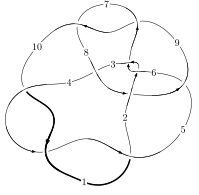
\includegraphics[width=112pt]{../../../GIT/diagram.site/Diagrams/png/178_10_94.png}\\
\ \ \ A knot diagram\footnotemark}&
\allowdisplaybreaks
\textbf{Linearized knot diagam} \\
\cline{2-2}
 &
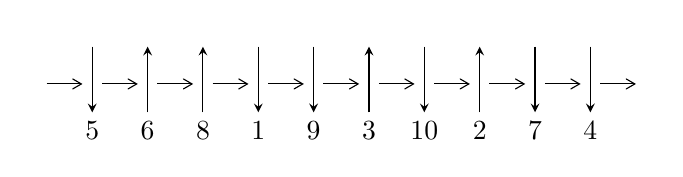
\begin{tikzpicture}[x=20pt, y=17pt]
	% nodes
	\node (C0) at (0, 0) {};
	\node (C1) at (1, 0) {};
	\node (C1U) at (1, +1) {};
	\node (C1D) at (1, -1) {5};

	\node (C2) at (2, 0) {};
	\node (C2U) at (2, +1) {};
	\node (C2D) at (2, -1) {6};

	\node (C3) at (3, 0) {};
	\node (C3U) at (3, +1) {};
	\node (C3D) at (3, -1) {8};

	\node (C4) at (4, 0) {};
	\node (C4U) at (4, +1) {};
	\node (C4D) at (4, -1) {1};

	\node (C5) at (5, 0) {};
	\node (C5U) at (5, +1) {};
	\node (C5D) at (5, -1) {9};

	\node (C6) at (6, 0) {};
	\node (C6U) at (6, +1) {};
	\node (C6D) at (6, -1) {3};

	\node (C7) at (7, 0) {};
	\node (C7U) at (7, +1) {};
	\node (C7D) at (7, -1) {10};

	\node (C8) at (8, 0) {};
	\node (C8U) at (8, +1) {};
	\node (C8D) at (8, -1) {2};

	\node (C9) at (9, 0) {};
	\node (C9U) at (9, +1) {};
	\node (C9D) at (9, -1) {7};

	\node (C10) at (10, 0) {};
	\node (C10U) at (10, +1) {};
	\node (C10D) at (10, -1) {4};
	\node (C11) at (11, 0) {};

	% arrows
	\draw[->,>={angle 60}]
	(C0) edge (C1) (C1) edge (C2) (C2) edge (C3) (C3) edge (C4) (C4) edge (C5) (C5) edge (C6) (C6) edge (C7) (C7) edge (C8) (C8) edge (C9) (C9) edge (C10) (C10) edge (C11) ;	\draw[->,>=stealth]
	(C1U) edge (C1D) (C2D) edge (C2U) (C3D) edge (C3U) (C4U) edge (C4D) (C5U) edge (C5D) (C6D) edge (C6U) (C7U) edge (C7D) (C8D) edge (C8U) (C9U) edge (C9D) (C10U) edge (C10D) ;
	\end{tikzpicture} \\
\hhline{~~} \\& 
\textbf{Solving Sequence} \\ \cline{2-2} 
 &
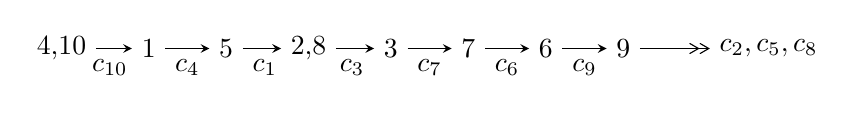
\begin{tikzpicture}[x=28pt, y=7pt]
	% node
	\node (A0) at (-1/8, 0) {4,10};
	\node (A1) at (1, 0) {1};
	\node (A2) at (2, 0) {5};
	\node (A3) at (49/16, 0) {2,8};
	\node (A4) at (33/8, 0) {3};
	\node (A5) at (41/8, 0) {7};
	\node (A6) at (49/8, 0) {6};
	\node (A7) at (57/8, 0) {9};
	\node (C1) at (1/2, -1) {$c_{10}$};
	\node (C2) at (3/2, -1) {$c_{4}$};
	\node (C3) at (5/2, -1) {$c_{1}$};
	\node (C4) at (29/8, -1) {$c_{3}$};
	\node (C5) at (37/8, -1) {$c_{7}$};
	\node (C6) at (45/8, -1) {$c_{6}$};
	\node (C7) at (53/8, -1) {$c_{9}$};
	\node (A8) at (9, 0) {$c_{2},c_{5},c_{8}$};

	% edge
	\draw[->,>=stealth]	
	(A0) edge (A1) (A1) edge (A2) (A2) edge (A3) (A3) edge (A4) (A4) edge (A5) (A5) edge (A6) (A6) edge (A7) ;
	\draw[->>,>={angle 60}]	
	(A7) edge (A8);
\end{tikzpicture} \\ 

\end{tabular} \\

\footnotetext{
The image of knot diagram is generated by the software ``\textbf{Draw programme}" developed by Andrew Bartholomew(\url{http://www.layer8.co.uk/maths/draw/index.htm\#Running-draw}), where we modified some parts for our purpose(\url{https://github.com/CATsTAILs/LinksPainter}).
}\phantom \\ \newline 
\centering \textbf{Ideals for irreducible components\footnotemark of $X_{\text{par}}$} 
 
\begin{align*}
I^u_{1}&=\langle 
-9.74096\times10^{15} u^{34}+8.22209\times10^{17} u^{33}+\cdots+6.62181\times10^{18} b+7.90428\times10^{18},\\
\phantom{I^u_{1}}&\phantom{= \langle  }-4.09728\times10^{18} u^{34}-3.86755\times10^{18} u^{33}+\cdots+6.62181\times10^{18} a-2.70054\times10^{18},\;u^{35}+3 u^{34}+\cdots+3 u^2-1\rangle \\
\\
\end{align*}
\raggedright * 1 irreducible components of $\dim_{\mathbb{C}}=0$, with total 35 representations.\\
\footnotetext{All coefficients of polynomials are rational numbers. But the coefficients are sometimes approximated in decimal forms when there is not enough margin.}
\newpage
\renewcommand{\arraystretch}{1}
\centering \section*{I. $I^u_{1}= \langle -9.74\times10^{15} u^{34}+8.22\times10^{17} u^{33}+\cdots+6.62\times10^{18} b+7.90\times10^{18},\;-4.10\times10^{18} u^{34}-3.87\times10^{18} u^{33}+\cdots+6.62\times10^{18} a-2.70\times10^{18},\;u^{35}+3 u^{34}+\cdots+3 u^2-1 \rangle$}
\flushleft \textbf{(i) Arc colorings}\\
\begin{tabular}{m{7pt} m{180pt} m{7pt} m{180pt} }
\flushright $a_{4}=$&$\begin{pmatrix}0\\u\end{pmatrix}$ \\
\flushright $a_{10}=$&$\begin{pmatrix}1\\0\end{pmatrix}$ \\
\flushright $a_{1}=$&$\begin{pmatrix}1\\u^2\end{pmatrix}$ \\
\flushright $a_{5}=$&$\begin{pmatrix}- u\\- u^3+u\end{pmatrix}$ \\
\flushright $a_{2}=$&$\begin{pmatrix}- u^2+1\\- u^4+2 u^2\end{pmatrix}$ \\
\flushright $a_{8}=$&$\begin{pmatrix}0.618755 u^{34}+0.584062 u^{33}+\cdots-9.67919 u+0.407825\\0.00147104 u^{34}-0.124167 u^{33}+\cdots+0.203436 u-1.19367\end{pmatrix}$ \\
\flushright $a_{3}=$&$\begin{pmatrix}1.09583 u^{34}+3.07364 u^{33}+\cdots-2.42964 u-5.58169\\-1.19271 u^{34}-2.87858 u^{33}+\cdots+1.54761 u+0.464135\end{pmatrix}$ \\
\flushright $a_{7}=$&$\begin{pmatrix}0.620226 u^{34}+0.459895 u^{33}+\cdots-9.47575 u-0.785850\\0.00147104 u^{34}-0.124167 u^{33}+\cdots+0.203436 u-1.19367\end{pmatrix}$ \\
\flushright $a_{6}=$&$\begin{pmatrix}2.14790 u^{34}+6.59302 u^{33}+\cdots-8.38643 u-4.87814\\-0.134603 u^{34}-0.623769 u^{33}+\cdots+1.93231 u-0.272284\end{pmatrix}$ \\
\flushright $a_{9}=$&$\begin{pmatrix}0.561562 u^{34}+0.370987 u^{33}+\cdots-9.79383 u+0.358105\\0.0974274 u^{34}+0.171295 u^{33}+\cdots+0.0892870 u-1.18951\end{pmatrix}$\\&\end{tabular}
\flushleft \textbf{(ii) Obstruction class $= -1$}\\~\\
\flushleft \textbf{(iii) Cusp Shapes $= \frac{28372200930047336304}{6621809224193386385} u^{34}+\frac{75749700395542932768}{6621809224193386385} u^{33}+\cdots-\frac{95288194958111912596}{6621809224193386385} u-\frac{24995006422002411154}{6621809224193386385}$}\\~\\
\newpage\renewcommand{\arraystretch}{1}
\flushleft \textbf{(iv) u-Polynomials at the component}\newline \\
\begin{tabular}{m{50pt}|m{274pt}}
Crossings & \hspace{64pt}u-Polynomials at each crossing \\
\hline $$\begin{aligned}c_{1},c_{4},c_{10}\end{aligned}$$&$\begin{aligned}
&u^{35}+3 u^{34}+\cdots+3 u^2-1
\end{aligned}$\\
\hline $$\begin{aligned}c_{2},c_{6}\end{aligned}$$&$\begin{aligned}
&u^{35}- u^{34}+\cdots-3 u^2+1
\end{aligned}$\\
\hline $$\begin{aligned}c_{3}\end{aligned}$$&$\begin{aligned}
&u^{35}+17 u^{34}+\cdots+214 u+23
\end{aligned}$\\
\hline $$\begin{aligned}c_{5}\end{aligned}$$&$\begin{aligned}
&u^{35}-13 u^{34}+\cdots+12 u-7
\end{aligned}$\\
\hline $$\begin{aligned}c_{7},c_{9}\end{aligned}$$&$\begin{aligned}
&u^{35}- u^{34}+\cdots-2 u+1
\end{aligned}$\\
\hline $$\begin{aligned}c_{8}\end{aligned}$$&$\begin{aligned}
&u^{35}-3 u^{34}+\cdots+4 u-1
\end{aligned}$\\
\hline
\end{tabular}\\~\\
\newpage\renewcommand{\arraystretch}{1}
\flushleft \textbf{(v) Riley Polynomials at the component}\newline \\
\begin{tabular}{m{50pt}|m{274pt}}
Crossings & \hspace{64pt}Riley Polynomials at each crossing \\
\hline $$\begin{aligned}c_{1},c_{4},c_{10}\end{aligned}$$&$\begin{aligned}
&y^{35}-37 y^{34}+\cdots+6 y-1
\end{aligned}$\\
\hline $$\begin{aligned}c_{2},c_{6}\end{aligned}$$&$\begin{aligned}
&y^{35}-21 y^{34}+\cdots+6 y-1
\end{aligned}$\\
\hline $$\begin{aligned}c_{3}\end{aligned}$$&$\begin{aligned}
&y^{35}-233 y^{34}+\cdots+5914 y-529
\end{aligned}$\\
\hline $$\begin{aligned}c_{5}\end{aligned}$$&$\begin{aligned}
&y^{35}-237 y^{34}+\cdots+942 y-49
\end{aligned}$\\
\hline $$\begin{aligned}c_{7},c_{9}\end{aligned}$$&$\begin{aligned}
&y^{35}-25 y^{34}+\cdots-70 y-1
\end{aligned}$\\
\hline $$\begin{aligned}c_{8}\end{aligned}$$&$\begin{aligned}
&y^{35}+3 y^{34}+\cdots+34 y-1
\end{aligned}$\\
\hline
\end{tabular}\\~\\
\newpage\flushleft \textbf{(vi) Complex Volumes and Cusp Shapes}
$$\begin{array}{c|c|c}  
\text{Solutions to }I^u_{1}& \I (\text{vol} + \sqrt{-1}CS) & \text{Cusp shape}\\
 \hline 
\begin{aligned}
u &= \phantom{-}0.638742 + 0.763228 I \\
a &= -0.32878 - 1.37864 I \\
b &= \phantom{-}1.265670 + 0.500696 I\end{aligned}
 & -0.17363 - 9.53352 I & -2.89594 + 8.02980 I \\ \hline\begin{aligned}
u &= \phantom{-}0.638742 - 0.763228 I \\
a &= -0.32878 + 1.37864 I \\
b &= \phantom{-}1.265670 - 0.500696 I\end{aligned}
 & -0.17363 + 9.53352 I & -2.89594 - 8.02980 I \\ \hline\begin{aligned}
u &= \phantom{-}0.421188 + 0.899484 I \\
a &= -0.792986 - 0.007441 I \\
b &= \phantom{-}1.102020 - 0.318172 I\end{aligned}
 & \phantom{-}0.51201 + 4.13357 I & -2.56649 - 6.25203 I \\ \hline\begin{aligned}
u &= \phantom{-}0.421188 - 0.899484 I \\
a &= -0.792986 + 0.007441 I \\
b &= \phantom{-}1.102020 + 0.318172 I\end{aligned}
 & \phantom{-}0.51201 - 4.13357 I & -2.56649 + 6.25203 I \\ \hline\begin{aligned}
u &= -0.708907 + 0.871150 I \\
a &= -0.370730 + 0.784435 I \\
b &= \phantom{-}1.164500 - 0.178894 I\end{aligned}
 & -3.73588 + 3.17966 I & -9.01884 - 7.80623 I \\ \hline\begin{aligned}
u &= -0.708907 - 0.871150 I \\
a &= -0.370730 - 0.784435 I \\
b &= \phantom{-}1.164500 + 0.178894 I\end{aligned}
 & -3.73588 - 3.17966 I & -9.01884 + 7.80623 I \\ \hline\begin{aligned}
u &= \phantom{-}0.555117 + 0.428217 I \\
a &= \phantom{-}1.29244 - 0.80829 I \\
b &= \phantom{-}0.267299 + 0.532419 I\end{aligned}
 & \phantom{-}2.98343 + 0.70642 I & \phantom{-}1.79862 + 1.96555 I \\ \hline\begin{aligned}
u &= \phantom{-}0.555117 - 0.428217 I \\
a &= \phantom{-}1.29244 + 0.80829 I \\
b &= \phantom{-}0.267299 - 0.532419 I\end{aligned}
 & \phantom{-}2.98343 - 0.70642 I & \phantom{-}1.79862 - 1.96555 I \\ \hline\begin{aligned}
u &= \phantom{-}0.420666 + 0.556962 I \\
a &= -0.213994 + 1.367610 I \\
b &= \phantom{-}0.122551 - 0.993553 I\end{aligned}
 & \phantom{-}3.42076 - 4.23935 I & \phantom{-}1.57284 + 6.50170 I \\ \hline\begin{aligned}
u &= \phantom{-}0.420666 - 0.556962 I \\
a &= -0.213994 - 1.367610 I \\
b &= \phantom{-}0.122551 + 0.993553 I\end{aligned}
 & \phantom{-}3.42076 + 4.23935 I & \phantom{-}1.57284 - 6.50170 I\\
 \hline 
 \end{array}$$\newpage$$\begin{array}{c|c|c}  
\text{Solutions to }I^u_{1}& \I (\text{vol} + \sqrt{-1}CS) & \text{Cusp shape}\\
 \hline 
\begin{aligned}
u &= -1.369300 + 0.067601 I \\
a &= \phantom{-}0.631419 - 0.279359 I \\
b &= \phantom{-}0.030418 + 0.167299 I\end{aligned}
 & -3.14805 + 0.11237 I & -2.00000 + 0. I\phantom{ +0.000000I} \\ \hline\begin{aligned}
u &= -1.369300 - 0.067601 I \\
a &= \phantom{-}0.631419 + 0.279359 I \\
b &= \phantom{-}0.030418 - 0.167299 I\end{aligned}
 & -3.14805 - 0.11237 I & -2.00000 + 0. I\phantom{ +0.000000I} \\ \hline\begin{aligned}
u &= \phantom{-}1.42805\phantom{ +0.000000I} \\
a &= -11.1085\phantom{ +0.000000I} \\
b &= -1.01279\phantom{ +0.000000I}\end{aligned}
 & -4.96247\phantom{ +0.000000I} & \phantom{-}155.290\phantom{ +0.000000I} \\ \hline\begin{aligned}
u &= -0.505143 + 0.260157 I \\
a &= \phantom{-}0.63134 - 1.66041 I \\
b &= -1.106350 + 0.599174 I\end{aligned}
 & -1.17815 + 2.75086 I & -5.83679 - 7.59594 I \\ \hline\begin{aligned}
u &= -0.505143 - 0.260157 I \\
a &= \phantom{-}0.63134 + 1.66041 I \\
b &= -1.106350 - 0.599174 I\end{aligned}
 & -1.17815 - 2.75086 I & -5.83679 + 7.59594 I \\ \hline\begin{aligned}
u &= \phantom{-}1.46072 + 0.11973 I \\
a &= -0.027998 + 0.767434 I \\
b &= -0.361779 - 0.871354 I\end{aligned}
 & -5.91469 - 2.99202 I & \phantom{-0.000000 } 0 \\ \hline\begin{aligned}
u &= \phantom{-}1.46072 - 0.11973 I \\
a &= -0.027998 - 0.767434 I \\
b &= -0.361779 + 0.871354 I\end{aligned}
 & -5.91469 + 2.99202 I & \phantom{-0.000000 } 0 \\ \hline\begin{aligned}
u &= -0.291602 + 0.421032 I \\
a &= \phantom{-}0.608613 - 0.956903 I \\
b &= -0.142845 + 0.366228 I\end{aligned}
 & -0.134869 + 1.085580 I & -2.08723 - 6.10429 I \\ \hline\begin{aligned}
u &= -0.291602 - 0.421032 I \\
a &= \phantom{-}0.608613 + 0.956903 I \\
b &= -0.142845 - 0.366228 I\end{aligned}
 & -0.134869 - 1.085580 I & -2.08723 + 6.10429 I \\ \hline\begin{aligned}
u &= -1.48666 + 0.16089 I \\
a &= -0.270075 - 0.598911 I \\
b &= -0.023905 + 1.336550 I\end{aligned}
 & -2.83088 + 6.77803 I & \phantom{-0.000000 } 0\\
 \hline 
 \end{array}$$\newpage$$\begin{array}{c|c|c}  
\text{Solutions to }I^u_{1}& \I (\text{vol} + \sqrt{-1}CS) & \text{Cusp shape}\\
 \hline 
\begin{aligned}
u &= -1.48666 - 0.16089 I \\
a &= -0.270075 + 0.598911 I \\
b &= -0.023905 - 1.336550 I\end{aligned}
 & -2.83088 - 6.77803 I & \phantom{-0.000000 } 0 \\ \hline\begin{aligned}
u &= -1.50842 + 0.01996 I \\
a &= -0.634805 - 0.360863 I \\
b &= -1.60295 + 0.26970 I\end{aligned}
 & -8.87322 + 0.26521 I & \phantom{-0.000000 } 0 \\ \hline\begin{aligned}
u &= -1.50842 - 0.01996 I \\
a &= -0.634805 + 0.360863 I \\
b &= -1.60295 - 0.26970 I\end{aligned}
 & -8.87322 - 0.26521 I & \phantom{-0.000000 } 0 \\ \hline\begin{aligned}
u &= \phantom{-}1.51371 + 0.06175 I \\
a &= -0.323814 + 0.778359 I \\
b &= -1.42288 - 0.85959 I\end{aligned}
 & -7.88737 - 3.84000 I & \phantom{-0.000000 } 0 \\ \hline\begin{aligned}
u &= \phantom{-}1.51371 - 0.06175 I \\
a &= -0.323814 - 0.778359 I \\
b &= -1.42288 + 0.85959 I\end{aligned}
 & -7.88737 + 3.84000 I & \phantom{-0.000000 } 0 \\ \hline\begin{aligned}
u &= \phantom{-}0.458527 + 0.023050 I \\
a &= -0.364039 + 0.257321 I \\
b &= -1.252630 - 0.041449 I\end{aligned}
 & -2.28660 - 0.00327 I & -6.71199 - 0.85350 I \\ \hline\begin{aligned}
u &= \phantom{-}0.458527 - 0.023050 I \\
a &= -0.364039 - 0.257321 I \\
b &= -1.252630 + 0.041449 I\end{aligned}
 & -2.28660 + 0.00327 I & -6.71199 + 0.85350 I \\ \hline\begin{aligned}
u &= -1.57609 + 0.25528 I \\
a &= \phantom{-}0.520584 + 1.107560 I \\
b &= \phantom{-}1.42500 - 0.57684 I\end{aligned}
 & -7.4557 + 13.3116 I & \phantom{-0.000000 } 0 \\ \hline\begin{aligned}
u &= -1.57609 - 0.25528 I \\
a &= \phantom{-}0.520584 - 1.107560 I \\
b &= \phantom{-}1.42500 + 0.57684 I\end{aligned}
 & -7.4557 - 13.3116 I & \phantom{-0.000000 } 0 \\ \hline\begin{aligned}
u &= \phantom{-}1.59602 + 0.26769 I \\
a &= \phantom{-}0.394220 - 0.908500 I \\
b &= \phantom{-}1.38166 + 0.35942 I\end{aligned}
 & -11.27950 - 7.30532 I & \phantom{-0.000000 } 0\\
 \hline 
 \end{array}$$\newpage$$\begin{array}{c|c|c}  
\text{Solutions to }I^u_{1}& \I (\text{vol} + \sqrt{-1}CS) & \text{Cusp shape}\\
 \hline 
\begin{aligned}
u &= \phantom{-}1.59602 - 0.26769 I \\
a &= \phantom{-}0.394220 + 0.908500 I \\
b &= \phantom{-}1.38166 - 0.35942 I\end{aligned}
 & -11.27950 + 7.30532 I & \phantom{-0.000000 } 0 \\ \hline\begin{aligned}
u &= -0.151482 + 0.347444 I \\
a &= \phantom{-}5.01455 - 1.87194 I \\
b &= -0.984898 - 0.180613 I\end{aligned}
 & -0.118043 - 0.668153 I & \phantom{-}2.12828 - 10.66433 I \\ \hline\begin{aligned}
u &= -0.151482 - 0.347444 I \\
a &= \phantom{-}5.01455 + 1.87194 I \\
b &= -0.984898 + 0.180613 I\end{aligned}
 & -0.118043 + 0.668153 I & \phantom{-}2.12828 + 10.66433 I \\ \hline\begin{aligned}
u &= -1.68110 + 0.33608 I \\
a &= \phantom{-}0.288307 + 0.479751 I \\
b &= \phantom{-}1.145510 - 0.065819 I\end{aligned}
 & -6.16860 + 1.10468 I & \phantom{-0.000000 } 0 \\ \hline\begin{aligned}
u &= -1.68110 - 0.33608 I \\
a &= \phantom{-}0.288307 - 0.479751 I \\
b &= \phantom{-}1.145510 + 0.065819 I\end{aligned}
 & -6.16860 - 1.10468 I & \phantom{-0.000000 } 0\\
 \hline 
 \end{array}$$\newpage
\newpage\renewcommand{\arraystretch}{1}
\centering \section*{ II. u-Polynomials}
\begin{tabular}{m{50pt}|m{274pt}}
Crossings & \hspace{64pt}u-Polynomials at each crossing \\
\hline $$\begin{aligned}c_{1},c_{4},c_{10}\end{aligned}$$&$\begin{aligned}
&u^{35}+3 u^{34}+\cdots+3 u^2-1
\end{aligned}$\\
\hline $$\begin{aligned}c_{2},c_{6}\end{aligned}$$&$\begin{aligned}
&u^{35}- u^{34}+\cdots-3 u^2+1
\end{aligned}$\\
\hline $$\begin{aligned}c_{3}\end{aligned}$$&$\begin{aligned}
&u^{35}+17 u^{34}+\cdots+214 u+23
\end{aligned}$\\
\hline $$\begin{aligned}c_{5}\end{aligned}$$&$\begin{aligned}
&u^{35}-13 u^{34}+\cdots+12 u-7
\end{aligned}$\\
\hline $$\begin{aligned}c_{7},c_{9}\end{aligned}$$&$\begin{aligned}
&u^{35}- u^{34}+\cdots-2 u+1
\end{aligned}$\\
\hline $$\begin{aligned}c_{8}\end{aligned}$$&$\begin{aligned}
&u^{35}-3 u^{34}+\cdots+4 u-1
\end{aligned}$\\
\hline
\end{tabular}\newpage\renewcommand{\arraystretch}{1}
\centering \section*{ III. Riley Polynomials}
\begin{tabular}{m{50pt}|m{274pt}}
Crossings & \hspace{64pt}Riley Polynomials at each crossing \\
\hline $$\begin{aligned}c_{1},c_{4},c_{10}\end{aligned}$$&$\begin{aligned}
&y^{35}-37 y^{34}+\cdots+6 y-1
\end{aligned}$\\
\hline $$\begin{aligned}c_{2},c_{6}\end{aligned}$$&$\begin{aligned}
&y^{35}-21 y^{34}+\cdots+6 y-1
\end{aligned}$\\
\hline $$\begin{aligned}c_{3}\end{aligned}$$&$\begin{aligned}
&y^{35}-233 y^{34}+\cdots+5914 y-529
\end{aligned}$\\
\hline $$\begin{aligned}c_{5}\end{aligned}$$&$\begin{aligned}
&y^{35}-237 y^{34}+\cdots+942 y-49
\end{aligned}$\\
\hline $$\begin{aligned}c_{7},c_{9}\end{aligned}$$&$\begin{aligned}
&y^{35}-25 y^{34}+\cdots-70 y-1
\end{aligned}$\\
\hline $$\begin{aligned}c_{8}\end{aligned}$$&$\begin{aligned}
&y^{35}+3 y^{34}+\cdots+34 y-1
\end{aligned}$\\
\hline
\end{tabular}
\vskip 2pc
\end{document}